\section{Scrapbook} \label{sec:Scrapbook}

\subsubsection*{Motivation} This pattern describes a way to make the project meaningful.  

\subsubsection*{Context} We have been working together for a while now.
We have maintained and revised our pattern catalog, and we are
achieving some of the ``What's Next'' steps associated with some of
the patterns.

\subsubsection*{Forces}~
\begin{tabular}[t]{p{.8\textwidth}@{\hspace{.03\textwidth}}c}
\textbf{Attention}: due to limited energy, we need to ask: where should we set the focus? &
%{\icon \symbol{"002168}}
\includegraphics{fire} \\
\textbf{Interest}: new experiences catch our attention. & 
%{\icon \symbol{"0021B9}}
\includegraphics{whale} \\
\textbf{Meaning}: shared history makes things meaningful. & 
%{\icon \symbol{"00214C}}
\includegraphics{museum} \\
\end{tabular}

\subsubsection*{Problem} Not all of the ideas we've come up with have proved workable.
Not all of the patterns we've noticed remain equally relevant.
In particular, some patterns no longer lead to concrete next steps.

\subsubsection*{Solution}
In order to maintain focus, is important to ``tune'' and ``prune'' the
things we give our attention to.  We can connect this understanding to
any actions undertaken in the project by asking questions like these:
%%%%%%%%%%%%%%%%%%%%%%%%%%%%%%%%%%%%%%%%%%%%%%%%%%%%%%%%%%%%%%%%%%%%%%%%%%%%%%%%%%%%%%%%%%%%%%%%%%%%
\begin{quote}
(1) Review what was supposed to happen.
(2) Establish what is happening/happened.
(3) Determine what’s right and wrong with what we are doing/have done.
(4) What did we learn or change? 
(5) What else should we change going forward?  \cite[Chapter 28]{peeragogy-handbook}, after \cite{afteraction}.
\end{quote}
%
%OSS: Who maintains the scrapbook? ... People say when you're learning, you should retain a learning log. Maybe scrapbook is like a shared notebook? All the process should be shared together, even if people take different paths, its all open. Journal of activities?
Other review processes have been formalized, including the design
review in architecture and the postmortem in theater and other
teamwork settings \cite{design-review,kerth2001project}.  The review
process may benefit from having an experienced facilitator on board
\cite[pp.~67, 142--143]{gabriel2002writer}.  As current priorities
become clearer, we decide where to focus.  Anything that isn't
receiving active attention should be moved to a
\patternname{Scrapbook}.  This may encompass:
\begin{itemize}
\item \emph{Retired patterns} that are tabled or completed (no more next steps);
\item \emph{Proto-patterns} made of problems, issues, and concerns;
\item \emph{A back-catalog} of publications, reports, or other
  artifacts.
\end{itemize}
In the Peeragogy project, alongside our patterns we initially
maintained a collection of antipatterns (like `\patternnameext{Magical
  thinking}') but the next steps coming from these seemed particularly
convoluted and abstract.  So, we archived
them.\footnote{\url{http://paragogy.net/Scrapbook}}  We present a
list of outstanding problems -- without known solutions -- right up
front in the Introduction to the \emph{Peeragogy Handbook}
\cite[Chapter 1]{peeragogy-handbook}.  Other proto-patterns include
`\patternnameext{Onboarding}' and `\patternnameext{Don't quit your day job}',
which arose in our review of this paper (see ``Emergent Roadmap'', below). 
Our back-catalog includes academic papers
\cite{building-peeragogy-accelerator,corneli2013inaction,corneli2012paragogical,paragogy-okcon}
and a thesis \cite{corneli-thesis}.
%
Everyone can maintain their own personal \patternname{Scrapbook} as
along with a communal one.  Furthermore, you don't need to limit
yourself to \emph{your own} creativity: include interesting ideas from
other sources (see \patternname{Reduce, reuse, recycle}). In some
cases a designated \patternname{Wrapper} may have to do further work
to elicit and organize contributions.

\subsubsection*{Rationale} 
We want to keep attention focused on the most relevant issues.  If a
pattern, task, or concern does not lead to concrete ``next steps'' at
the moment, sufficient time for reflection may offer a better
understanding, and it may prove useful and actionable in a different
context.

\subsubsection*{Resolution} 
Judicious use of the \patternname{Scrapbook} can help focus project participants' \textbf{attention} on current concerns, without losing grasp of items of \textbf{interest}.  The currently active pattern catalog is leaner and more action-oriented as a result. If the \patternname{Roadmap} shows where we're going, it is the \patternname{Scrapbook} that shows most clearly where we've been, and collects the observations that are most \textbf{meaningful} to us.

\subsubsection*{Example 1} 
The history of the Wikimedia Foundation, and of Wiki\-pedia, are
maintained as wiki
pages.\footnote{\url{https://wikimediafoundation.org/wiki/History_of_the_Wikimedia_Foundation}}\textsuperscript{,}\footnote{\url{https://en.wikipedia.org/wiki/Wikipedia}}
One of the entries on Wikipedia details outstanding issues, in the
form of
critiques.\footnote{\url{https://en.wikipedia.org/wiki/Criticism_of_Wikipedia}}
There are many tools available 
to help facilitate the process of
vetting proposed fine-grained changes to
articles.\footnote{\url{https://en.wikipedia.org/wiki/Special:RecentChanges}}\textsuperscript{,}\footnote{\url{https://en.wikipedia.org/wiki/Wikipedia:Recent_changes_patrol\#Tools}}
Policy concerns are typically discussed at the Village Pump, and 
there are mechanisms in place for settling
disputes.\footnote{\url{https://en.wikipedia.org/wiki/Wikipedia:Village_pump_(policy)}}\textsuperscript{,}\footnote{\url{https://en.wikipedia.org/wiki/Wikipedia:Requests_for_comment}}

%\begin{wrapfigure}{r}{.47\textwidth}
%\vspace{-.2cm}
\begin{figure}
\begin{center}
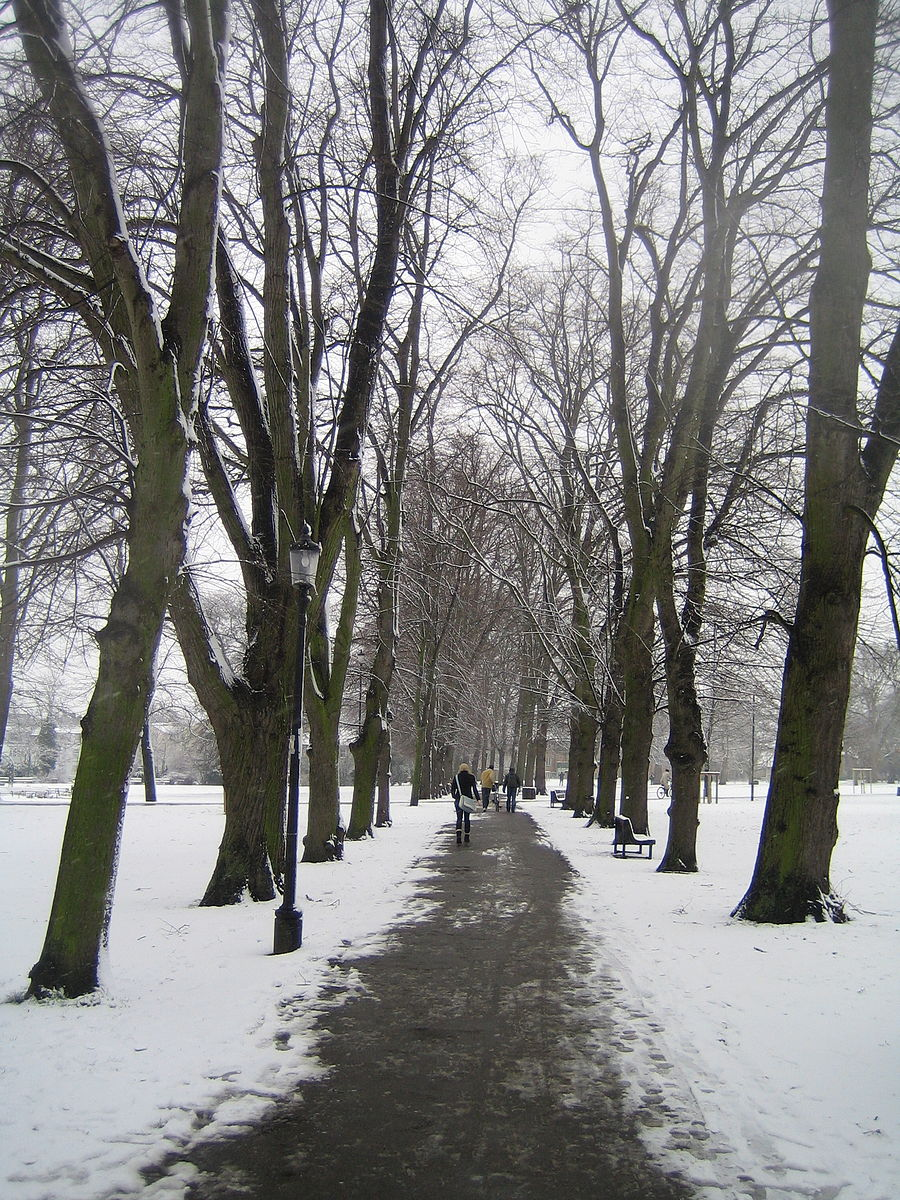
\includegraphics[width=\textwidth,trim=0 325 0 500, clip=true]{ChristsPieces}
\end{center}
\vspace{-.4cm}
\captionsetup{font=footnotesize,width=.47\textwidth}
\caption{\textsl{Park}: Christ's Pieces, Cambridge, UK.
% Public domain.
\label{christs-pieces}}
\end{figure}
%\vspace{-1.1cm}
%\end{wrapfigure}

\subsubsection*{Example 2} 
Just as a university campus grows and changes over time, future
peeragogues will be drawn to new problems and patterns. They
will trace new paths and build new emergent structures (Figure
\ref{christs-pieces}).

\smallskip

\begin{framed}
\noindent 
\emph{What's Next in the Peeragogy Project}
\definecollection{ScrapbookWN}
\begin{collectinmacro}{\ScrapbookWN}{}{}
After pruning back our pattern catalog, we want it to grow again: new patterns are needed.
One strategy would be to turn the whole \emph{Peeragogy Handbook} into design patterns.
\end{collectinmacro}
\ScrapbookWN
\end{framed}


%\newpage
